\documentclass[tikz,border=10pt]{standalone}
\usepackage{tkz-euclide} % 增强几何绘图功能

\begin{document}
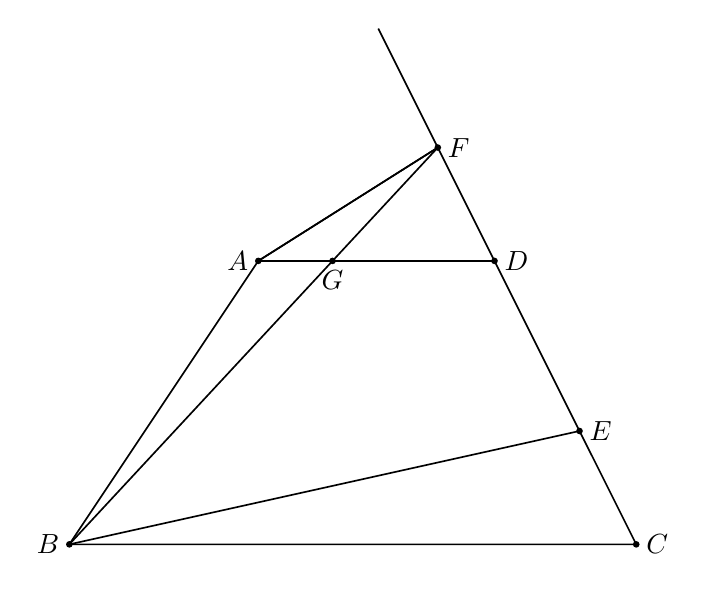
\begin{tikzpicture}[scale=1.2, line width=0.6pt, >=stealth]
    % 1. 定义核心顶点坐标 (根据图像比例估算)
    \coordinate (B) at (0, 0);
    \coordinate (C) at (6, 0);
    \coordinate (A) at (2, 3);
    \coordinate (D) at (4.5, 3); % 确保 AD 平行于 BC
    
    % 2. 计算延长线上的点 F (在 CD 延长线上)
    % 设定 F 在 CD 向量方向上的延长位置
    \coordinate (F) at ($(D)!-0.4!(C)$); 
    
    % 3. 定义点 E (在线段 CD 上)
    \coordinate (E) at ($(D)!0.6!(C)$);
    
    % 4. 计算交点 G (线段 BF 与 线段 AD 的交点)
    \coordinate (G) at (intersection of B--F and A--D);
    
    % 5. 绘制主要轮廓线
    \draw (A) -- (B) -- (C) -- (F) -- cycle; % 绘制外围主体
    \draw (A) -- (D); % 绘制梯形上底
    
    % 6. 绘制内部连接线
    \draw (B) -- (F); % 连结 BF，经过 G
    \draw (B) -- (E); % 连结 BE
    \draw (A) -- (F); % 连结 AF
    
    % 7. 绘制 F 点上方的延伸线 (示意直线性质)
    \draw (F) -- ($(F)!-0.3!(C)$);

    % 8. 标注点名称
    % anchor 用于微调文字位置，避免覆盖线段
    \node[left] at (A) {$A$};
    \node[left] at (B) {$B$};
    \node[right] at (C) {$C$};
    \node[right] at (D) {$D$};
    \node[right] at (E) {$E$};
    \node[right] at (F) {$F$};
    \node[below] at (G) {$G$};

    % 9. 可选：绘制点的小圆点（增加视觉清晰度）
    \foreach \p in {A,B,C,D,E,F,G}
        \fill (\p) circle (1pt);

\end{tikzpicture}
\end{document}